% ============================================================================
% Ablation of the multimodal update (simulation) -- proposed Sec. V-B.4
% Requires: booktabs, graphicx.  Figures: fig_ablation_modes.pdf (double
% column), fig_ablation_tau.pdf (single column).
% Data: results/scenario_b/main_20261012{,_s10_19}, results/scenario_b/fig5_static
% ============================================================================

\subsubsection{Ablation of the Multimodal Update}
\label{sec:ablation}

To isolate the contribution of the multimodal update, we compare BM2PC with two ablated variants that differ from it in a single component. All variants use the obstacle-avoidance configuration of Table~\ref{tab:sim_params} ($H=35$, $N=402$ samples per iteration, $I=1$, $\sigma=1.5$, $\lambda^{-1}=850$, $K=200$, filtering threshold $10^5$, $\pm 5$\,m/s$^2$, 40\,Hz), i.e., the same rollout budget and execution conditions:
\begin{itemize}
\item \textbf{BM2PC} ($n=3$, $\beta=600$): the proposed method.
\item \textbf{$n=1$}: a single control mode; all $N$ samples are drawn around one center, and the next center is the candidate with the highest posterior score in the same filtered top-$K$ pool. The diversity term vanishes.
\item \textbf{$\beta=0$}: three modes without diversity reward. With $\beta=0$, the incremental objective~\eqref{eq:f_inc} reduces to the posterior score, so the greedy update returns the three highest-scoring candidates. This variant therefore coincides with cost-only top-$n$ retention up to the prior term.
\end{itemize}

\textbf{Static obstacle.} We first repeat the obstacle-avoidance task of Fig.~\ref{fig:sim_obstacle} with 10 random seeds per variant (40 obstacle crossings each). All three variants pass the obstacle without contact in every crossing and reach almost identical tracking accuracy (RMSE 6.2, 6.5, and 6.3\,cm averaged over seeds; Table~\ref{tab:ablation}). This is expected: with replanning at 40\,Hz and a 0.875\,s horizon, even a single mode re-converges to a collision-free solution before reaching a static obstacle. Maintaining multiple modes matters when the currently preferred solution \emph{suddenly} becomes infeasible, which motivates the following scenario.

\textbf{Sudden blocking scenario.} The rope tip tracks a back-and-forth straight pass $\bm{p}^{\mathrm{ref}}(t)=[0,\;0.9(1-\cos\omega t),\;0.2]^\top$\,m with a peak speed of 1.2\,m/s, reached at the midpoint, where a cylindrical pillar A (radius 5\,cm, inflated by 2\,cm for planning, as in Sec.~\ref{sec:sim_obstacle}) is placed. Pillar A is extended in height (0.05--1.05\,m) so that the rope cannot pass over it, which leaves exactly two homotopy classes, left and right, whose nominal costs are equal by symmetry. At a lead time $\tau$ before the reference reaches pillar A, an identical pillar B appears tangent to A on the side through which the predicted rope-tip trajectory of the executed mode passes. Pillar B therefore always blocks the channel preferred by the evaluated controller, and the controller must switch to the opposite channel. Pillar B is removed 0.6\,s after the reference passes A. As in the other experiments, the planner receives the current obstacle positions at every control step without any motion prediction. Each 12\,s episode contains four crossings (the first crossing is excluded as a start-up transient). We sweep $\tau\in\{0.60,0.65,\dots,0.85\}$\,s with 10 seeds per value (20 seeds for $\tau\ge 0.75$\,s), giving 40 or 80 blocking events per variant and lead time. We also run the same pass without pillar B (\emph{symmetric static}).

An event is counted as a \emph{success} if the rope tip passes pillar A by at least 10\,cm within 1\,s after the reference crossing without any rope--pillar contact, checked at every 1\,kHz simulation step. Failed events are either \emph{collisions} (any contact) or \emph{stalls} (no contact, but the tip does not get past the pillars). We additionally report the maximum tip tracking error within the event window. Success rates are given with 95\% Wilson intervals and compared with Fisher's exact test.

\begin{table}[t]
\centering
\caption{Ablation of the multimodal update (simulation). Succ.: collision-free passage of pillar A (\%). Sudden-blocking results are pooled over $\tau\in[0.70,0.85]$\,s (280 events per variant).}
\label{tab:ablation}
\footnotesize
\setlength{\tabcolsep}{2.6pt}
\begin{tabular}{@{}lcccccccc@{}}
\toprule
& \multicolumn{2}{c}{Fig.~\ref{fig:sim_obstacle} scene} & \multicolumn{2}{c}{Symmetric static} & \multicolumn{4}{c}{Sudden blocking} \\
\cmidrule(lr){2-3}\cmidrule(lr){4-5}\cmidrule(l){6-9}
Variant & Succ. & RMSE & Succ. & RMSE & Succ. & Coll. & Stall & Max err. \\
&       & (cm) &       & (cm) &       & (\%)  & (\%)  & (cm)     \\
\midrule
BM2PC ($n{=}3$) & \textbf{100} & 6.2 & \textbf{95.0} & \textbf{10.5} & \textbf{72.1} & \textbf{20.0} & \textbf{7.9} & \textbf{50.4} \\
$n{=}1$         & \textbf{100} & 6.5 & 85.0 & 19.8 & 50.7 & 33.6 & 15.7 & 72.8 \\
$\beta{=}0$     & \textbf{100} & 6.3 & 77.5 & 30.4 & 52.1 & 30.4 & 17.5 & 71.3 \\
\bottomrule
\end{tabular}
\end{table}

\begin{figure}[t]
\centering
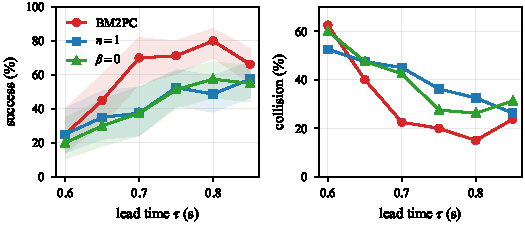
\includegraphics[width=\columnwidth]{fig_ablation_tau.pdf}
\caption{Sudden blocking: success rate (95\% Wilson interval shaded) and collision rate versus the lead time $\tau$ at which pillar B appears.}
\label{fig:ablation_tau}
\end{figure}

\begin{figure*}[t]
\centering
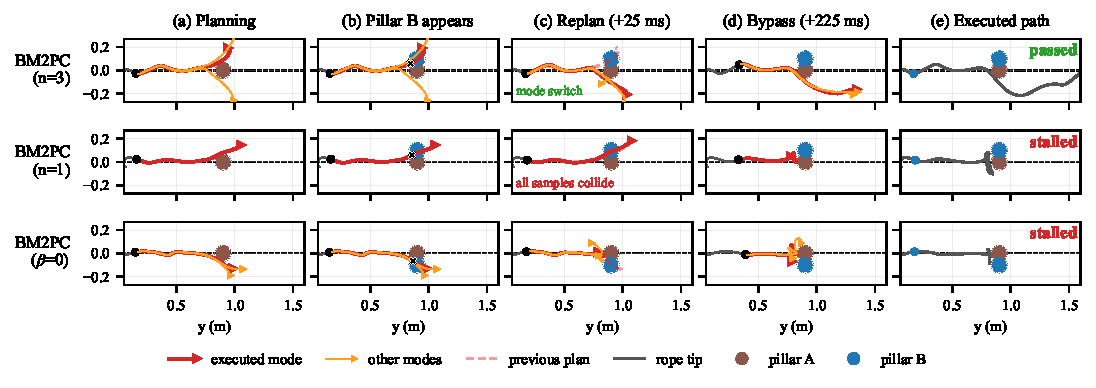
\includegraphics[width=\textwidth]{fig_ablation_modes.pdf}
\caption{Sudden blocking, one event ($\tau=0.70$\,s, same seed for all variants), top view (horizontal axis $y$, vertical axis $x$, in meters); the dashed line is the reference, pillar A is fixed, and pillar B appears. (a)~Predicted rope-tip trajectories of the control modes at the step at which pillar B appears. (b)~The same plan with pillar B overlaid: the executed plan of every variant runs into B ($\times$: first point inside the inflated pillar). (c)~First replan that observes B (+25\,ms): BM2PC switches to the mode that already passes on the free side, whereas for $n=1$ all samples collide and the $\beta=0$ modes remain clustered in front of the pillars. (d)~+225\,ms: BM2PC bypasses the pillars, while the ablated variants still fail to find a solution on the free side. (e)~Executed rope-tip paths up to 1\,s after the reference passes pillar A (the evaluation window); BM2PC returns to the reference after the bypass.}
\label{fig:ablation_modes}
\end{figure*}

\textbf{Results.} Table~\ref{tab:ablation} and Fig.~\ref{fig:ablation_tau} summarize the results. In the sudden-blocking scenario with $\tau\in[0.70,0.85]$\,s, BM2PC passes the pillars in 72.1\% of the events, compared with 50.7\% for $n=1$ and 52.1\% for $\beta=0$ ($p<10^{-5}$ for both comparisons). It also reduces the collision rate from 33.6\% and 30.4\% to 20.0\%, halves the stall rate, and lowers the maximum tracking error from about 72\,cm to 50\,cm. The difference is significant at $\tau=0.70$, 0.75, and 0.80\,s individually ($p<0.03$), and BM2PC attains the highest or an equal success rate at every lead time. For $\tau\le0.65$\,s, all variants mostly fail (at most 45\% success): by then the rope has committed to one side, and the opposite channel can hardly be reached within the remaining time. For $\tau=0.85$\,s, pillar B appears close to the end of the horizon, which leaves enough time for single-mode replanning, and the gap narrows. Even without pillar B, the symmetric configuration favors BM2PC (95.0\% vs.\ 85.0\% and 77.5\% success, 10.5 vs.\ 19.8 and 30.4\,cm RMSE).

Fig.~\ref{fig:ablation_modes} illustrates the mechanism. Before pillar B appears, BM2PC keeps one mode on each side of pillar A, although the executed mode passes on the side that is about to be blocked. When B appears, the alternative mode is already available and becomes the executed one at the next replanning step. In contrast, the samples of the $n=1$ variant are concentrated around a single center: all of them collide after B appears, and local sampling around the blocked plan does not reach the free channel within the remaining time. Similarly, the $\beta=0$ variant retains three nearly identical candidates, so it loses all of its modes at once. Quantitatively, at the moment pillar B appears, BM2PC holds a mode on the free side in 57\% of the events (160/280), and in these events it switches channel in 74\% of the cases, compared with 57\% when no such mode is present. The remaining failures of BM2PC are mainly contacts during the aggressive evasive maneuver, likely because the 2\,cm planning margin is small relative to the mismatch between the planning model and the simulated rope.

These results show that the multimodal update does not merely reproduce what a single, frequently replanned mode achieves. Its benefit appears when the preferred solution suddenly becomes infeasible. Both components are required: maintaining several modes ($n>1$) and the diversity reward ($\beta>0$), without which the retained modes collapse to the same solution.
